\documentclass[a4paper]{article}
\usepackage{times}
\usepackage[utf8]{inputenc}
\usepackage{selinput}
\usepackage{upquote}
\usepackage[margin=2cm, rmargin=4cm, tmargin=3cm]{geometry}
\usepackage{tcolorbox}
\usepackage{xspace}
\usepackage[french]{babel}
\usepackage{url}
\usepackage{hyperref}
\usepackage{fontawesome5}
\usepackage{marginnote}
\usepackage{ulem}
\usepackage{tcolorbox}
\usepackage{graphicx}
%\usepackage[top=Bcm, bottom=Hcm, outer=Ccm, inner=Acm, heightrounded, marginparwidth=Ecm, marginparsep=Dcm]{geometry}


\newtcolorbox{Example}[1]{colback=white,left=20pt,colframe=slideblue,fonttitle=\bfseries,title=#1}
\newtcolorbox{Solutions}[1]{colback=white,left=20pt,colframe=green,fonttitle=\bfseries,title=#1}
\newtcolorbox{Conseils}[1]{colback=white,left=20pt,colframe=slideblue,fonttitle=\bfseries,title=#1}
\newtcolorbox{Warning}[1]{colback=white,left=20pt,colframe=warning,fonttitle=\bfseries,title=#1}

\setlength\parindent{0pt}

  %Exercice environment
  \newcounter{exercice}
  \newenvironment{Exercice}[1][]
  {
  \par
  \stepcounter{exercice}\textbf{Question \arabic{exercice}:} (\faClock \enskip \textit{#1})
  }
  {\bigskip}
  

% Title
\newcommand{\titre}{\begin{center}
  \section*{Algorithmes et Pensée Computationnelle}
\end{center}}
\newcommand{\cours}[1]
{\begin{center} 
  \textit{#1}\\
\end{center}
  }


\newcommand{\exemple}[1]{\newline~\textbf{Exemple :} #1}
%\newcommand{\attention}[1]{\newline\faExclamationTriangle~\textbf{Attention :} #1}

% Documentation url (escape \# in the TP document)
\newcommand{\documentation}[1]{\faBookOpen~Documentation : \href{#1}{#1}}

% Clef API
\newcommand{\apikey}[1]{\faKey~Clé API : \lstinline{#1}}
\newcommand{\apiendpoint}[1]{\faGlobe~Url de base de l'API \href{#1}{#1}}

%Listing Python style
\usepackage{color}
\definecolor{slideblue}{RGB}{33,131,189}
\definecolor{green}{RGB}{0,190,100}
\definecolor{blue}{RGB}{121,142,213}
\definecolor{grey}{RGB}{120,120,120}
\definecolor{warning}{RGB}{235,186,1}

\usepackage{listings}
\lstdefinelanguage{texte}{
    keywordstyle=\color{black},
    numbers=none,
    frame=none,
    literate=
           {é}{{\'e}}1
           {è}{{\`e}}1
           {ê}{{\^e}}1
           {à}{{\`a}}1
           {â}{{\^a}}1
           {ù}{{\`u}}1
           {ü}{{\"u}}1
           {î}{{\^i}}1
           {ï}{{\"i}}1
           {ë}{{\"e}}1
           {Ç}{{\,C}}1
           {ç}{{\,c}}1,
    columns=fullflexible,keepspaces,
	breaklines=true,
	breakatwhitespace=true,
}
\lstset{
    language=Python,
	basicstyle=\bfseries\footnotesize,
	breaklines=true,
	breakatwhitespace=true,
	commentstyle=\color{grey},
	stringstyle=\color{slideblue},
  keywordstyle=\color{slideblue},
	morekeywords={with, as, True, False, Float, join, None, main, argparse, self, sort, __eq__, __add__, __ne__, __radd__, __del__, __ge__, __gt__, split, os, endswith, is_file, scandir, @classmethod},
	deletekeywords={id},
	showspaces=false,
	showstringspaces=false,
	columns=fullflexible,keepspaces,
	literate=
           {é}{{\'e}}1
           {è}{{\`e}}1
           {ê}{{\^e}}1
           {à}{{\`a}}1
           {â}{{\^a}}1
           {ù}{{\`u}}1
           {ü}{{\"u}}1
           {î}{{\^i}}1
           {ï}{{\"i}}1
           {ë}{{\"e}}1
           {Ç}{{\,C}}1
           {ç}{{\,c}}1,
    numbers=left,
}

\newtcbox{\mybox}{nobeforeafter,colframe=white,colback=slideblue,boxrule=0.5pt,arc=1.5pt, boxsep=0pt,left=2pt,right=2pt,top=2pt,bottom=2pt,tcbox raise base}
\newcommand{\projet}{\mybox{\textcolor{white}{\small projet}}\xspace}
\newcommand{\optionnel}{\mybox{\textcolor{white}{\small Optionnel}}\xspace}
\newcommand{\advanced}{\mybox{\textcolor{white}{\small Pour aller plus loin}}\xspace}
\newcommand{\auto}{\mybox{\textcolor{white}{\small Auto-évaluation}}\xspace}


\usepackage{environ}
\newif\ifShowSolution
\NewEnviron{solution}{
  \ifShowSolution
	\begin{Solutions}{\faTerminal \enskip Solution}
		\BODY
	\end{Solutions}
  \fi}


  \usepackage{environ}
  \newif\ifShowConseil
  \NewEnviron{conseil}{
    \ifShowConseil
    \begin{Conseils}{\faLightbulb \quad Conseil}
      \BODY
    \end{Conseils}

    \fi}

    \usepackage{environ}
  \newif\ifShowWarning
  \NewEnviron{attention}{
    \ifShowWarning
    \begin{Warning}{\faExclamationTriangle \quad Attention}
      \BODY
    \end{Warning}

    \fi}
  

%\newcommand{\Conseil}[1]{\ifShowIndice\ \newline\faLightbulb[regular]~#1\fi}


\usepackage{array}
\usepackage{blindtext}
\usepackage{multicol}
\newcolumntype{C}[1]{>{\centering\let\newline\\\arraybackslash\hspace{0pt}}m{#1}}

\begin{document}
% Change the following values to true to show the solutions or/and the hints
\ShowSolutiontrue
\ShowConseiltrue
\ShowNotefalse
\titre
\cours{Consolidation 2}

Les exercices de cette série sont une compilation d'exercices semblables à ceux vus lors des semaines précédentes. Le but de cette séance est de consolider les connaissances acquises lors des travaux pratiques des dernière semaines.\\

% Exercice complexité - Maeva
\begin{Exercice}[10 minutes] \textbf{Complexité} \\
	Analysez la complexité des deux programmes ci-dessous. Ont-ils la même complexité? 
    	\lstinputlisting{resources/ex1_enonce.py}

	% Solutions complexité - Maeva
	\begin{solution}
	Non, ils n'ont pas la même complexité. \lstinline{fun()} a une complexité de $O(n*n)$ car il s'agit de deux boucles imbriquées itérant chacune n fois dans le pire des cas. En revanche, \lstinline{fun2()} a une complexité de $O(n+n)$ car elle contient deux boucles effectuant des opérations indépendantes. 
	\end{solution}
\end{Exercice}

\begin{comment}
% Exercice complexité - Maeva
\begin{Exercice}[10 minutes]\textbf{Complexité}\\
	Quel est la complexité de ce code ?
   	 \lstinputlisting{resources/ex2_enonce.py}
	 % Exercice complexité - Maeva
	 \begin{solution}
		%TODO 
	\end{solution}
\end{Exercice}
\end{comment}

% Exercice nombres impaire - Maeva
\begin{Exercice}[10 minutes] \textbf{Programmation de base}\\
	Ecrivez un programme Python qui imprime tous les nombres impairs à partir de 1 jusqu’à un nombre \lstinline{n} défini par l’utilisateur. Ce nombre \lstinline{n} doit être supérieur à 1.
	Exemple : si n = 6, résultat attendu : 1, 3, 5
% Solutions nombres impaire - Maeva
	\begin{solution}
   		 \lstinputlisting{solutions/exercise3.py}
	\end{solution}
\end{Exercice}

% Exercice arbres binaires - Maeva
\begin{Exercice}[10 minutes] \textbf{Arbres binaires} \\
	Lesquels de ces arbres sont des arbres binaires de recherche (binary search tree) ? Donnez leur hauteur (height).
	
	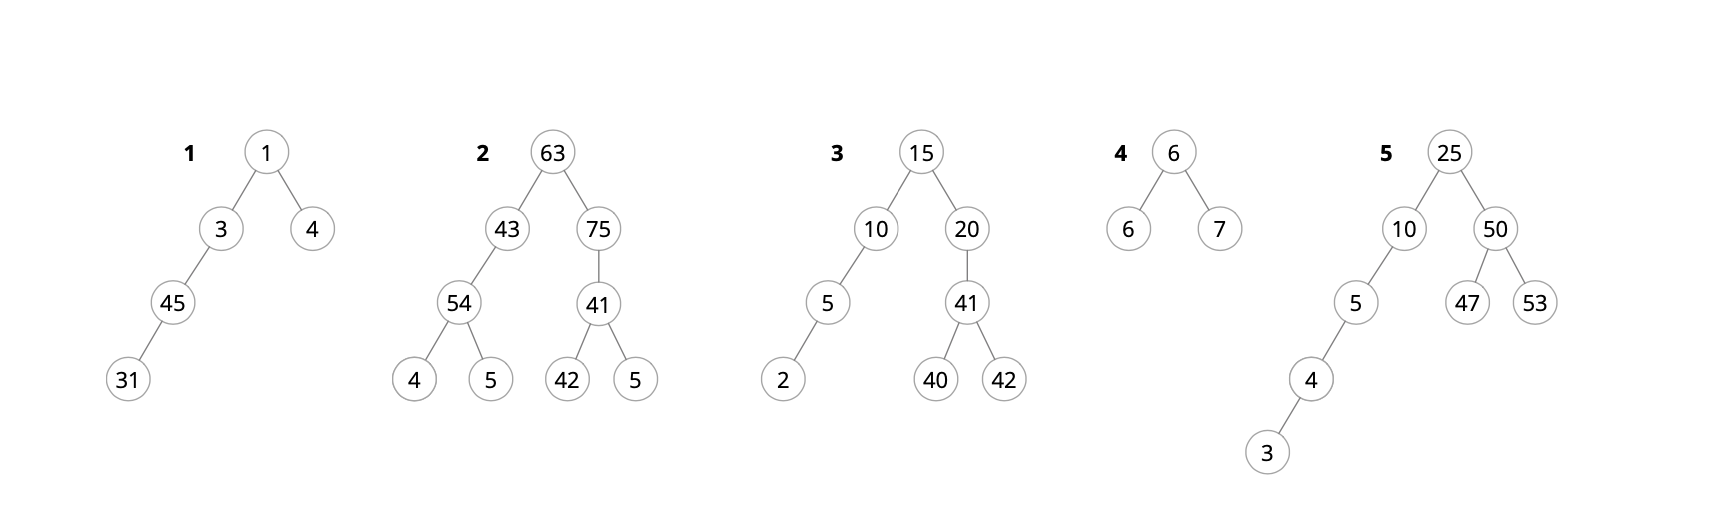
\includegraphics[width=18cm]{resources/exercice5.png}

	% Solution arbres binaires - Maeva
	\begin{solution}
		Seuls les arbres 3, 4 et 5 sont des arbres binaires de recherche selon la définition donnée en cours. En effet, l'ordre d'insertion des éléments est incorrect dans les arbres 1 et 2. 
		Quant à leurs hauteurs, elles sont respectivement de 3, 3, 3, 1 et 4.
	\end{solution}
\end{Exercice}


% Exercice théorique - Etienne
\begin{Exercice}[20 minutes]\textbf{Arbres binaires}\\
	\begin{enumerate}
		\item Ecrire un programme Python ayant une complexité temporelle de $O(log n)$ et qui prend comme argument un tableau trié \lstinline{A[1, ..., n]} de $n$ nombres et une clé $k$. Ce programme devra retourner \textbf{"OUI"} si \lstinline{A} contient $k$ et \textbf{"NON"} dans le cas contraire.
		\item Quelle est la hauteur minimale et la hauteur maximale d'un arbre binaire de recherche ayant $n$ éléments? Exprimer votre réponse en fonction du nombre de noeuds $n$ présents dans l'arbre.
		\item Considerer l'arbre binaire suivant : \\
		
		Dessiner les arbres obtenus après execution de chacune des opérations suivantes (chaque opération~est exécutée en commençant par l'arbre ci-dessus - les opérations ne sont pas exécutées de façon séquentielle).
		
		\begin{figure}[h!]
        			\centering
       	 		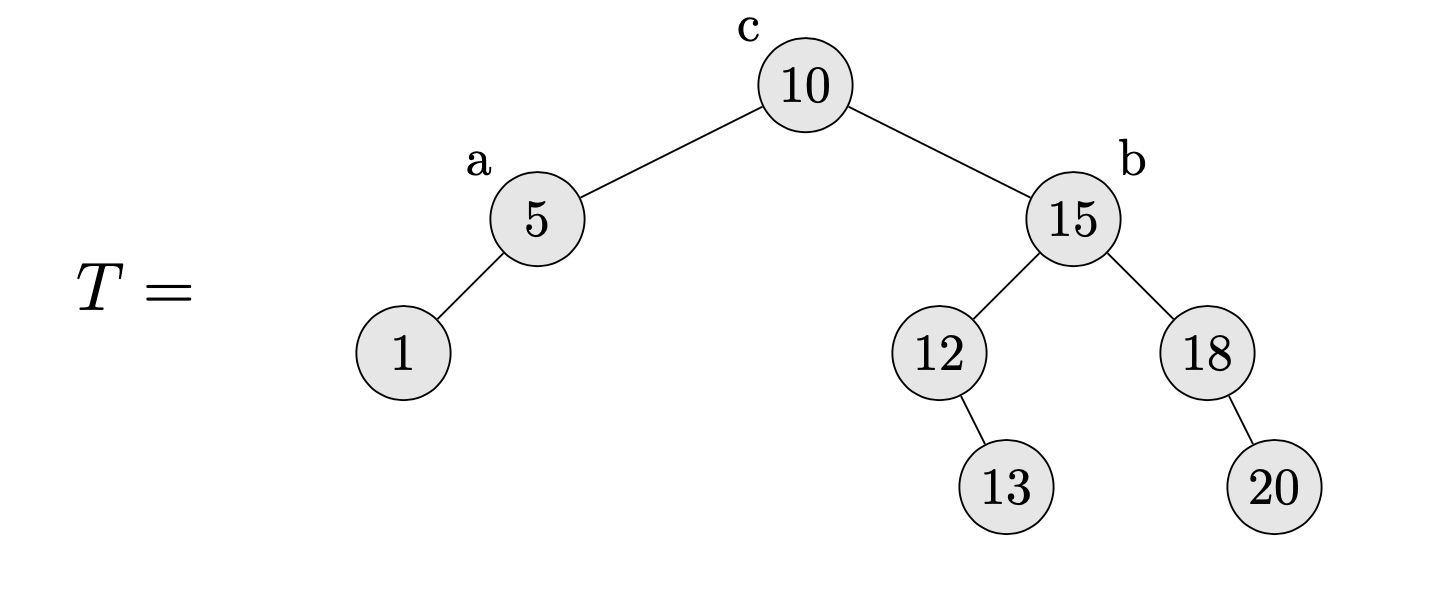
\includegraphics[width=10cm]{resources/exoArbreBinEnonce.png}
	    	\end{figure}
		\begin{enumerate}
			\item \textsc{Tree-Insert}(T, z) avec z.key = 0
			\item \textsc{Tree-Insert}(T, z) avec z.key = 17
			\item \textsc{Tree-Insert}(T, z) avec z.key = 14
			\item \textsc{Tree-Delete}(T, a)
			\item \textsc{Tree-Delete}(T, b)
			\item \textsc{Tree-Delete}(T, c)
		\end{enumerate}


	\end{enumerate}
	% Solution exercice théorique - Etienne
	\begin{solution}
		\begin{enumerate}
			\item Etant donné que les nombres du tableau A sont triés, nous utilisons l'algorithme de recherche binaire. L'algorithme de recherche binaire  prend comme argument un tableau A, une clé k, des indices p et q et retourne "OUI" si A[p . . . q]  contient la clé k et "NON" autrement. Comme A[p . . . q] est trié, nous pouvons comparer k avec l'élément du milieu mid = $\lfloor(p+q)//2\rfloor$  et : \\
				\begin{itemize}
					\item Si A[mid] = k return "OUI" \\
					\item Si A[mid] $>$ k, alors cherchons k dans le tableau A[p . . . (mid-1)] en appelant récursivement l'algorithme \textsc{Binary-Search}(A, k, p, mid-1) \\
					\item Si A[mid] $<$ k, alors cherchons k dans le tableau A[(mid + 1) . . . q] en appelant récursivement l'algorithme \textsc{Binary-Search}(A, k, mid+1, q)\\
				\end{itemize}
				Le programme permettant d'effectuer une recherche binaire est le suivant:
				\lstinputlisting{solutions/exerciseTheorieBinarySearch.py}
			\item Hauteur minimale et maximale d'un arbre binaire.
				\begin{itemize}
					\item La hauteur maximale d'un arbre binaire est atteinte quand l'arbre n'est constitué que d'une seule branche. \\
					
						%\begin{figure}[h!]
        						%	\centering
       	 					%	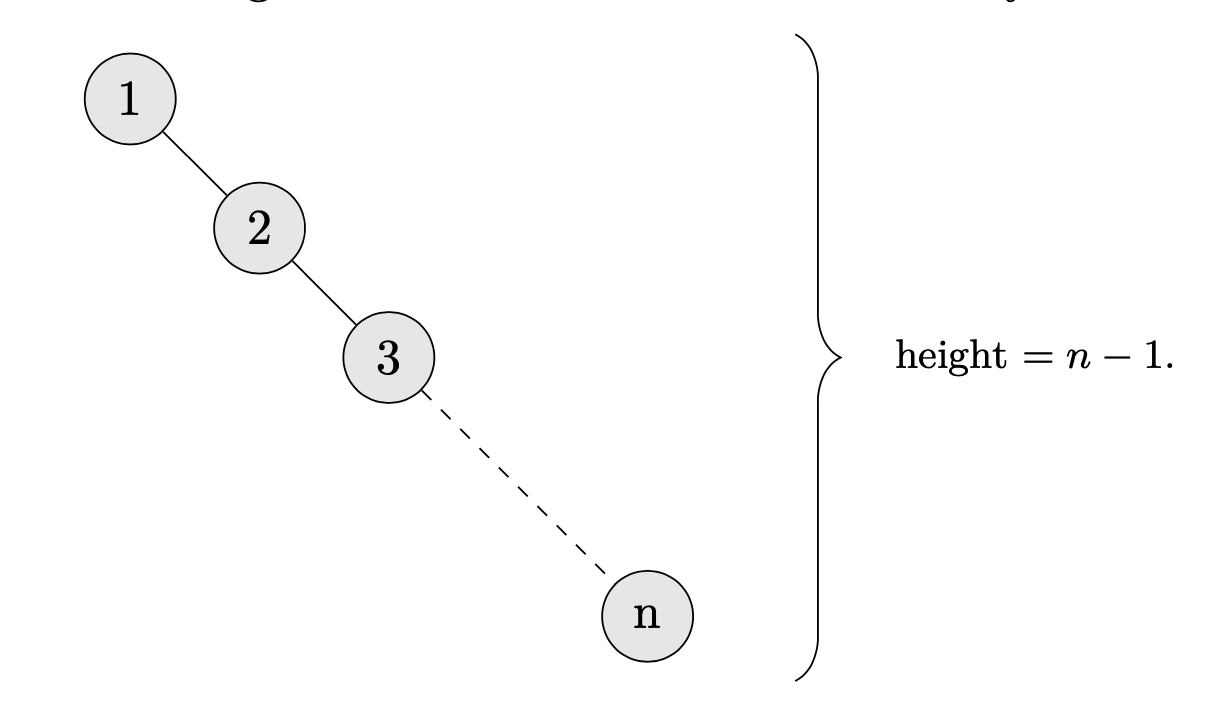
\includegraphics[width=6cm]{solutions/maxHeight.png}
	    					%\end{figure}
					\item La hauteur minimale est atteinte lorsque l'arbre binaire est ``complet'' : nous ne pouvons pas ajouter de noeud sans augmenter la hauteur de l'arbre hauteur de un. \\
        							\centering
       	 						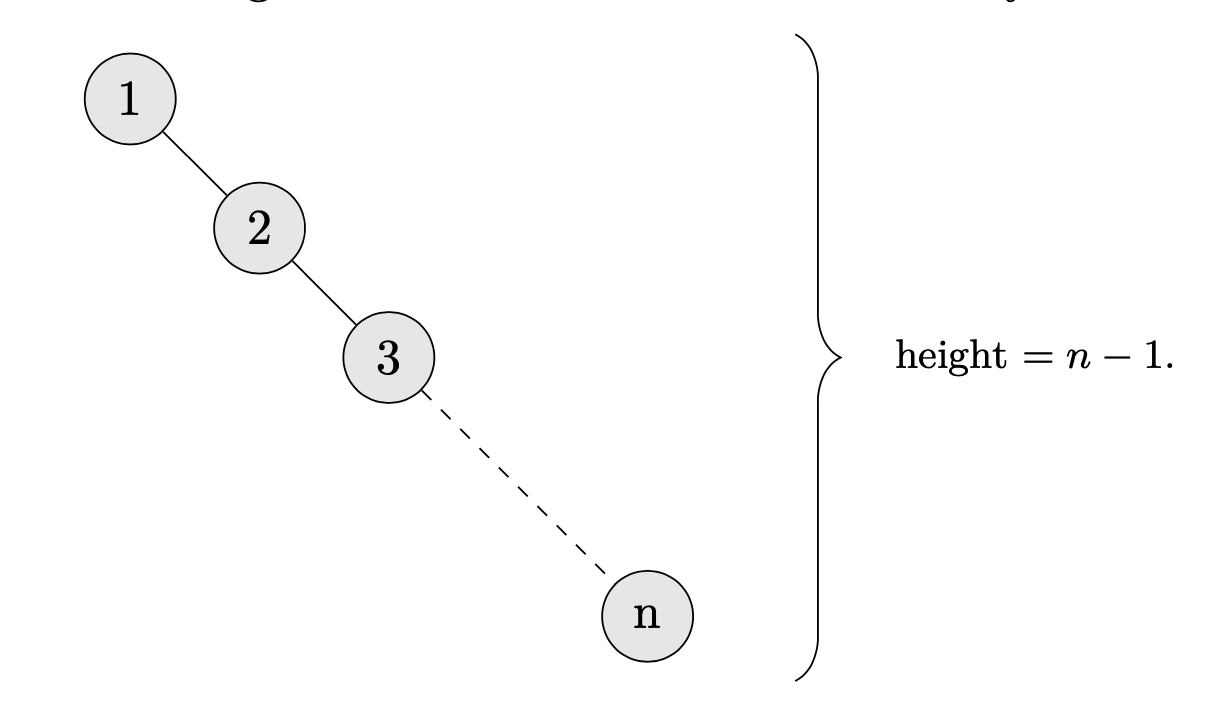
\includegraphics[width=6cm]{solutions/maxHeight.png}
       	 						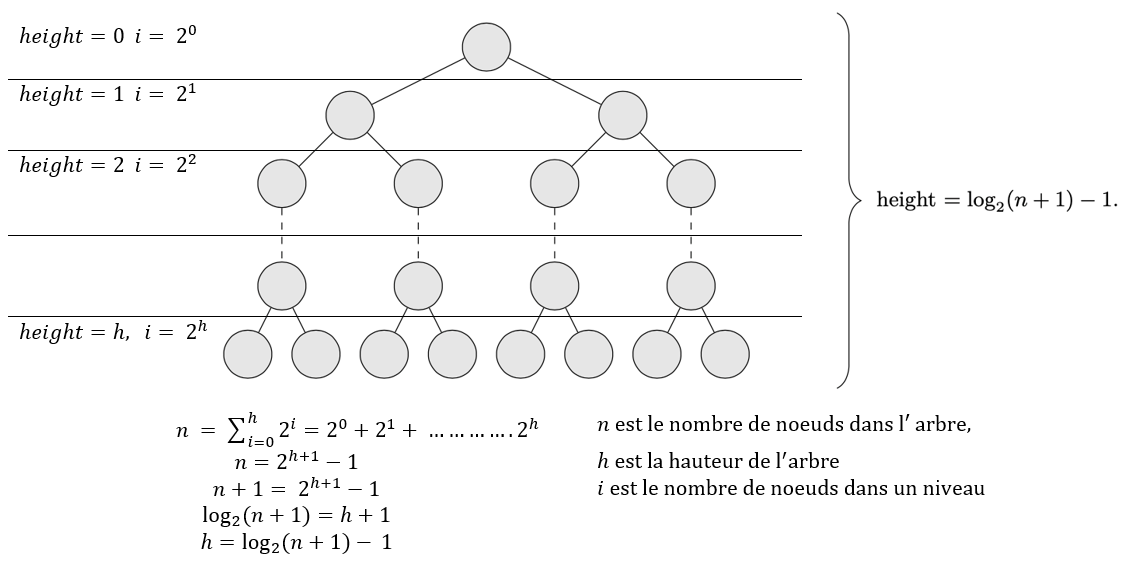
\includegraphics[width=12cm]{solutions/minHeight.png}
				\end{itemize}
			\item Après execution de chaque opération, nous obtenons:

		\end{enumerate}
	\end{solution}

	\begin{solution}
			\begin{enumerate}
				\item Figure A : \textsc{Tree-Insert}(T, z) avec z.key = 0
				\item Figure B : \textsc{Tree-Insert}(T, z) avec z.key = 17
				\item Figure C: \textsc{Tree-Insert}(T, z) avec z.key = 14
				\item Figure D : \textsc{Tree-Delete}(T, a)
				\item Figure E : \textsc{Tree-Delete}(T, b)
				\item Figure F : \textsc{Tree-Delete}(T, c)
			\end{enumerate}
		\centering
		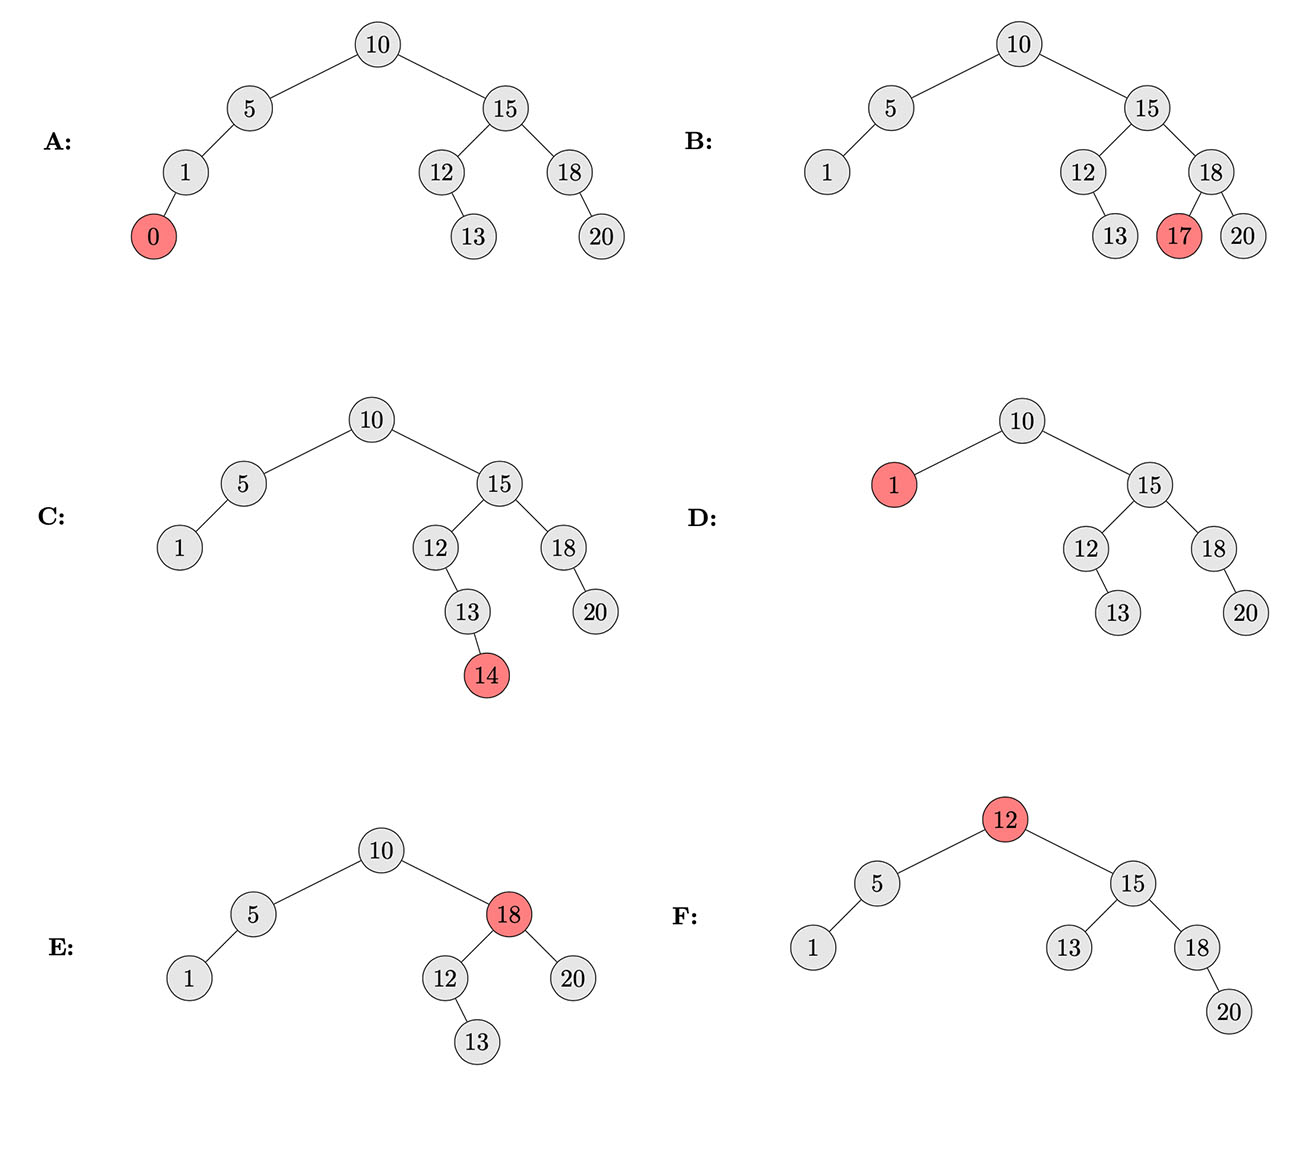
\includegraphics[width=9cm]{solutions/tree_merged.jpg}
	\end{solution}
		
\end{Exercice}

% Exercice complexité - Etienne
\begin{Exercice}[10 minutes]\textbf{Croissance de fonctions}\\
	Nous avons vu comment exprimer la complexité d'un algorithme en terme de complexité temporelle dans le ``\emph{pire des cas}'', notée $\mathcal{O}$(). L'exercice suivant permet de travailler avec différentes croissances de fonctions.\\ Ordonner la liste de fonctions suivante selon leur croissance asymptotique: il faut trier les fonctions par ordre croissant de notation grand-$\mathcal{O}$. La notation grand-$\mathcal{O}$() donne une borne supérieure du taux de croissance d'une fonction. Ainsi si $f(x) = 2x$ et $g(x) = 3x^2$, on dit que que $f(x)$ équivaut à $\mathcal{O}(x)$ et que $g(x)$ équivaut à $\mathcal{O}(x^2)$. On peut alors les ordonner pour obtenir : $\mathcal{O}(f(x)) < \mathcal{O}(g(x)) \Leftrightarrow \mathcal{O}(x) < \mathcal{O}(x^2)$.
	
		\begin{equation}
			n^{\sqrt{n}}, n\cdot log(n), n^{1/log(n)}, log(log(n)), \sqrt{n}, 3^{n}/{n^5}, 2^n
		\end{equation}
		
		% Solutions complexité - Etienne
		\begin{solution}
			\begin{itemize}
				\item D'abord la constante : $n^{1/log(n)} = (2^{log(n)})^{1/log(n)}$
				\item Ensuite le $log(log(n))$
				\item Puis $n^{\sqrt{n}} = 2^{\sqrt{n}\cdot log_2(n)}$
				\item Puis $2^n$
				\item Enfin  $3^{n}/{n^5}$
			\end{itemize}
		\end{solution}
	\end{Exercice}
	


% Exercice BFS Papier - Sarra
\begin{Exercice}[10 minutes]\textbf{Breadth-First Search : Papier
}\\
\\
	Le but du Breadth-First Search (BFS) ou algorithme de parcours en largeur est d'explorer un graphe à partir d’un sommet donné (sommet de départ ou sommet source). \\

	Appliquez l’algorithme \lstinline{BFS} au graphe suivant en partant du sommet B:\\

	\begin{figure}[h!]
        		\centering
       	 	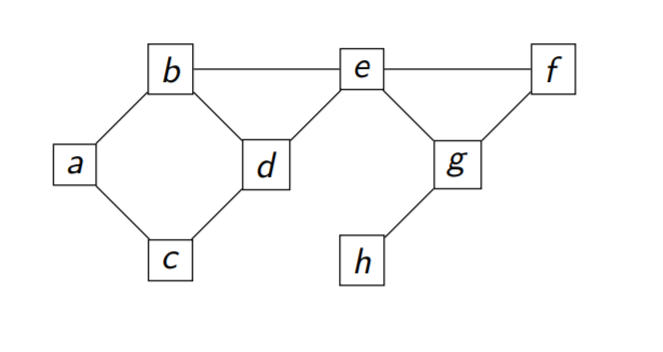
\includegraphics[width = 9cm]{resources/exerciceBFS.png}
	\end{figure}


	% Solution BFS - Sarra
	\begin{solution}
Dans cette solution, nous considèrons le sommet $b$ comme sommet de départ et l'ordre alphabétique dans l'exploration des voisins.\\

		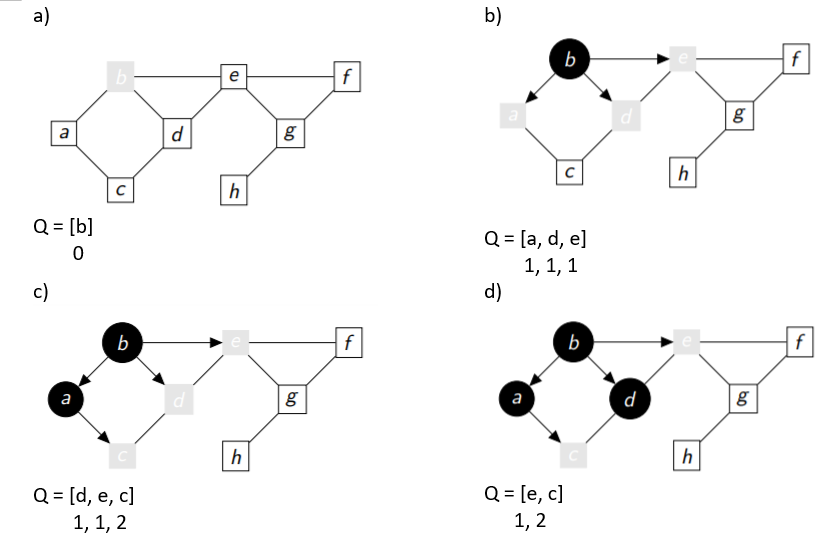
\includegraphics[width=8cm]{solutions/BFS1.PNG}\\
		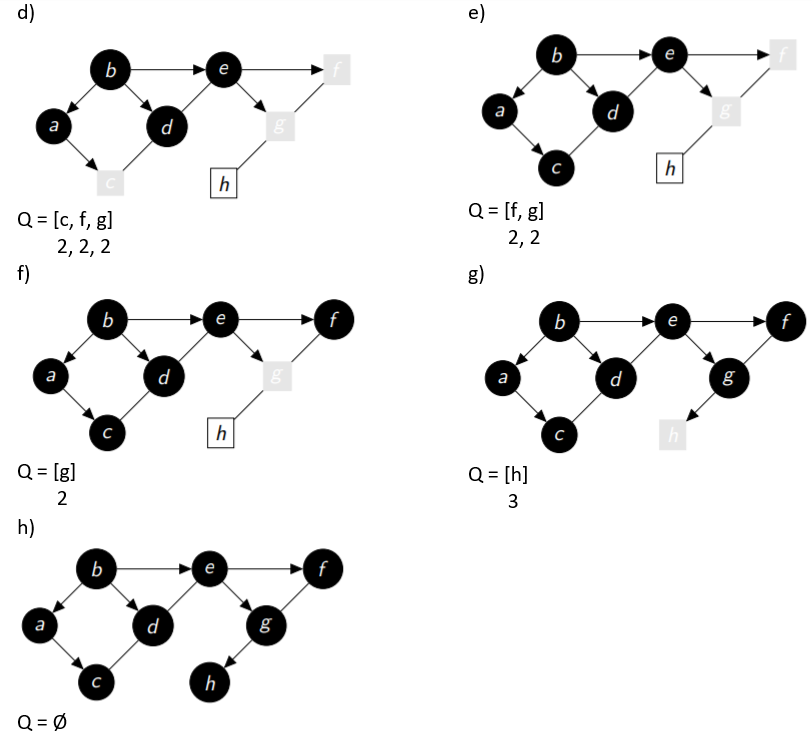
\includegraphics[width=8cm]{solutions/BFS2.PNG}\\
 		Ci-dessous l'arborescence associée au parcours.\\
		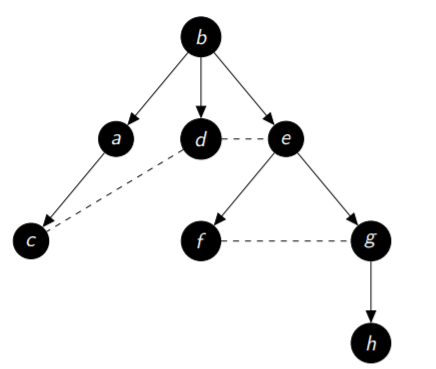
\includegraphics[width=5cm]{solutions/BFS3.PNG}\\
		L’ordre de parcours est : ligne après ligne (de la racine vers les feuilles) et
		de gauche à droite pour une ligne ($b, a, d, e, c, f, g, h$).
	\end{solution}
\end{Exercice}

% Exercice BFS Python - Sarra
\begin{Exercice}[15 minutes]\textbf{Breadth-First Search : Python
}\\
	Dans cet exercice, nous aimerions identifier le chemin le plus court entre deux nœuds d'un graphe.
	La fonction que nous implémentons doit pouvoir accepter comme argument un graphe, un nœud de départ et un nœud de fin. Si l'algorithme est capable de connecter les nœuds 			de départ et d'arrivée, il doit renvoyer le chemin parcouru. Nous allons utiliser l'algorithme BFS car il renvoie toujours le chemin le plus court dans un graphe non pondéré (dont le poids entre tous les nœuds est inexistant ou virtuellement égal à 1).
	    Implémentez l'algorithme en suivant les étapes suivantes :\\
	\begin{enumerate}
	    
		\item Partir du sommet initial, construire un chemin avec le premier nœud et le mettre dans une \textbf{queue}.
		\item Extraire le premier chemin de la \textbf{queue} et récupérer le dernier nœud du chemin. Si ce nœud n'a pas été visité, parcourir ses sommets adjacents (voisins). Pour chaque voisin construire un nouveau chemin et le mettre dans la \textbf{queue}.
		\item Ajouter le nœud à la liste des nœuds \textbf{visités}. Une fois que cela est fait, supprimer le chemin  parcouru de la queue.
		\item Répéter les étapes 2 et 3 jusqu'à ce que la queue soit vide ou le nœud d'arrivée est atteint.\\
	\end{enumerate}

	\lstinputlisting[language=python]{resources/bfs_enonce.py}
    	\begin{conseil}
		Il existe quelques différences principales entre l'implémentation de BFS et  l'application du plus court chemin.
		
        		\begin{enumerate}
			\item La file d'attente garde une trace des chemins possibles (implémentés sous forme de liste de nœuds) au lieu des nœuds.
	           	\item lorsque l'algorithme recherche un nœud voisin, il doit vérifier si le nœud voisin correspond au nœud cible. Si c'est le cas, nous avons une solution et il n'est pas 					nécessaire de continuer à explorer le graphique.
        		\end{enumerate}

    	\end{conseil}

	% Solution BFS - Sarra
	\begin{solution}
		\lstinputlisting{solutions/bfs_shortest_path.py}
	\end{solution}
\end{Exercice}

% Exercice Kruskal Papier - Sarra
\begin{Exercice}[10 minutes] \textbf{Algorithme de Kruskal : Papier}\\
\\
    	Appliquez l'algorithme de Kruskal au graphe suivant :\\
	
	\centering
    	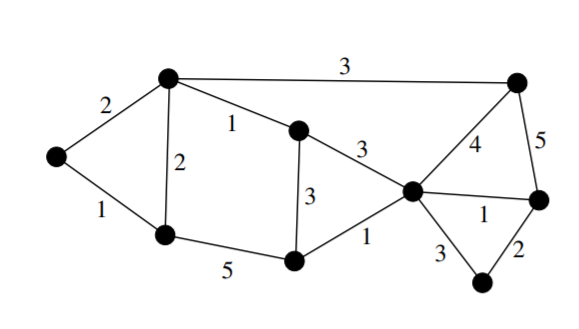
\includegraphics[]{resources/exerciceKruskal.PNG}
    	\begin{conseil}
        		L'algorithme de Kruskal fonctionne de la façon suivante :
        		\begin{enumerate}
		            \item Classer les arêtes par ordre croissant de poids.
		            \item Prendre l'arête avec le poids le plus faible et l'ajouter à l'arbre (si 2 arêtes ont le même poids, choisir arbitrairement une des 2).
		            \item Vérifiez que l'arête ajoutée ne crée pas de cycle, si c'est le cas, supprimez la.
		            \item Répétez les étapes 2) et 3) jusqu'à ce que tous les sommets aient été atteints.
	        \end{enumerate}
	        Un Minimum Spanning Tree, s'il existe, a toujours un nombre d'arêtes égal au nombre de sommets moins un. Par exemple, ici notre graphe a 9 sommets. L'algorithme devrait donc 			s'arrêter lorsque 8 arêtes ont été choisies.
    	\end{conseil}
    \begin{solution}
        Vous trouverez ci-dessous les étapes de la construction du MST(Minimum spanning tree) avec l'algorithme de Kruskal :\\
        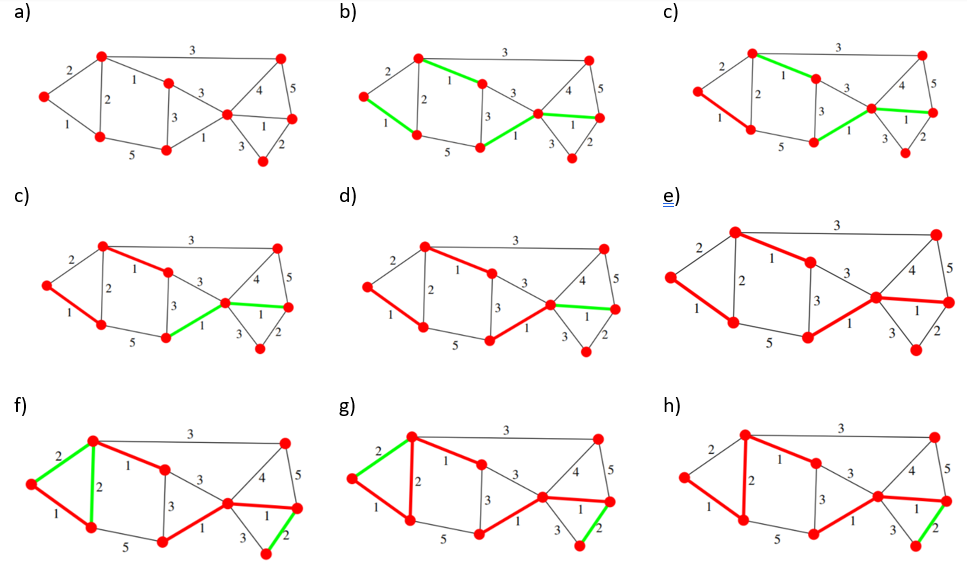
\includegraphics[width=13cm]{solutions/K1.PNG}\\
        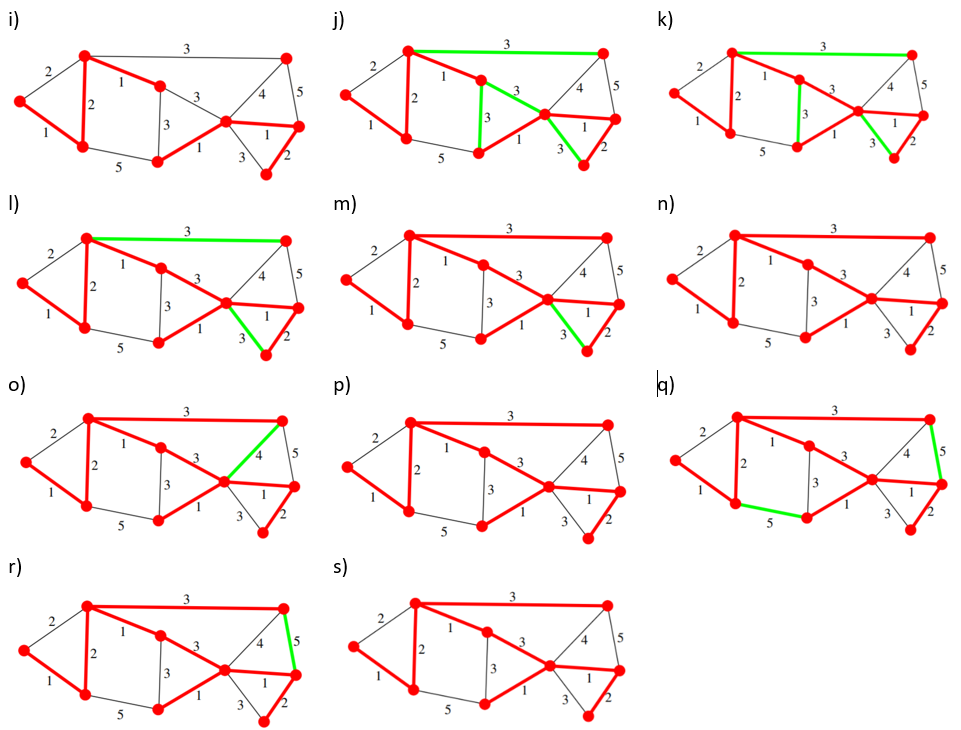
\includegraphics[width=13cm]{solutions/K2.PNG}\\
        L'algorithme s'arrête car tous les sommets ont été atteints. On voit bien que seules 8 arêtes ont été nécessaires.
      
    \end{solution}

\end{Exercice}

\end{document}